\documentclass[a3paper,landscape]{article}
\usepackage[margin=1cm]{geometry}
\usepackage{tikz}
\usetikzlibrary{positioning, arrows.meta, fit, calc}

% ── Class box style ──
\tikzset{
  class/.style={
    draw, rectangle, rounded corners=2pt,
    fill=blue!5, minimum width=3.4cm,
    font=\footnotesize, inner sep=4pt,
    align=left
  },
  classname/.style={
    font=\footnotesize\bfseries, align=center
  },
  sep line/.style={
    draw, thin, gray
  },
  inherit/.style={
    -{Triangle[open, length=6pt, width=6pt]}, thick
  },
  compose/.style={
    -{Diamond[open, length=6pt, width=5pt]}, thick
  },
  assoc/.style={
    -{Stealth[length=5pt]}, thick
  },
  label style/.style={
    font=\tiny, fill=white, inner sep=1pt
  },
  module label/.style={
    font=\scriptsize\bfseries\itshape, text=blue!60!black
  }
}

% ── Macro to draw a class box ──
\newcommand{\umlclass}[4][]{%
  % #1 = tikz node name, #2 = class title, #3 = attributes, #4 = methods
  \node[class, #1] {
    \begin{tabular}{l}
      \multicolumn{1}{c}{\textbf{#2}} \\
      \hline
      #3 \\
      \hline
      #4 \\
    \end{tabular}
  };
}

\begin{document}
\pagestyle{empty}

\begin{center}
{\LARGE\bfseries CampVerse — UML Class Diagram}\\[4pt]
{\small Campus Management System}
\end{center}

\vspace{2mm}

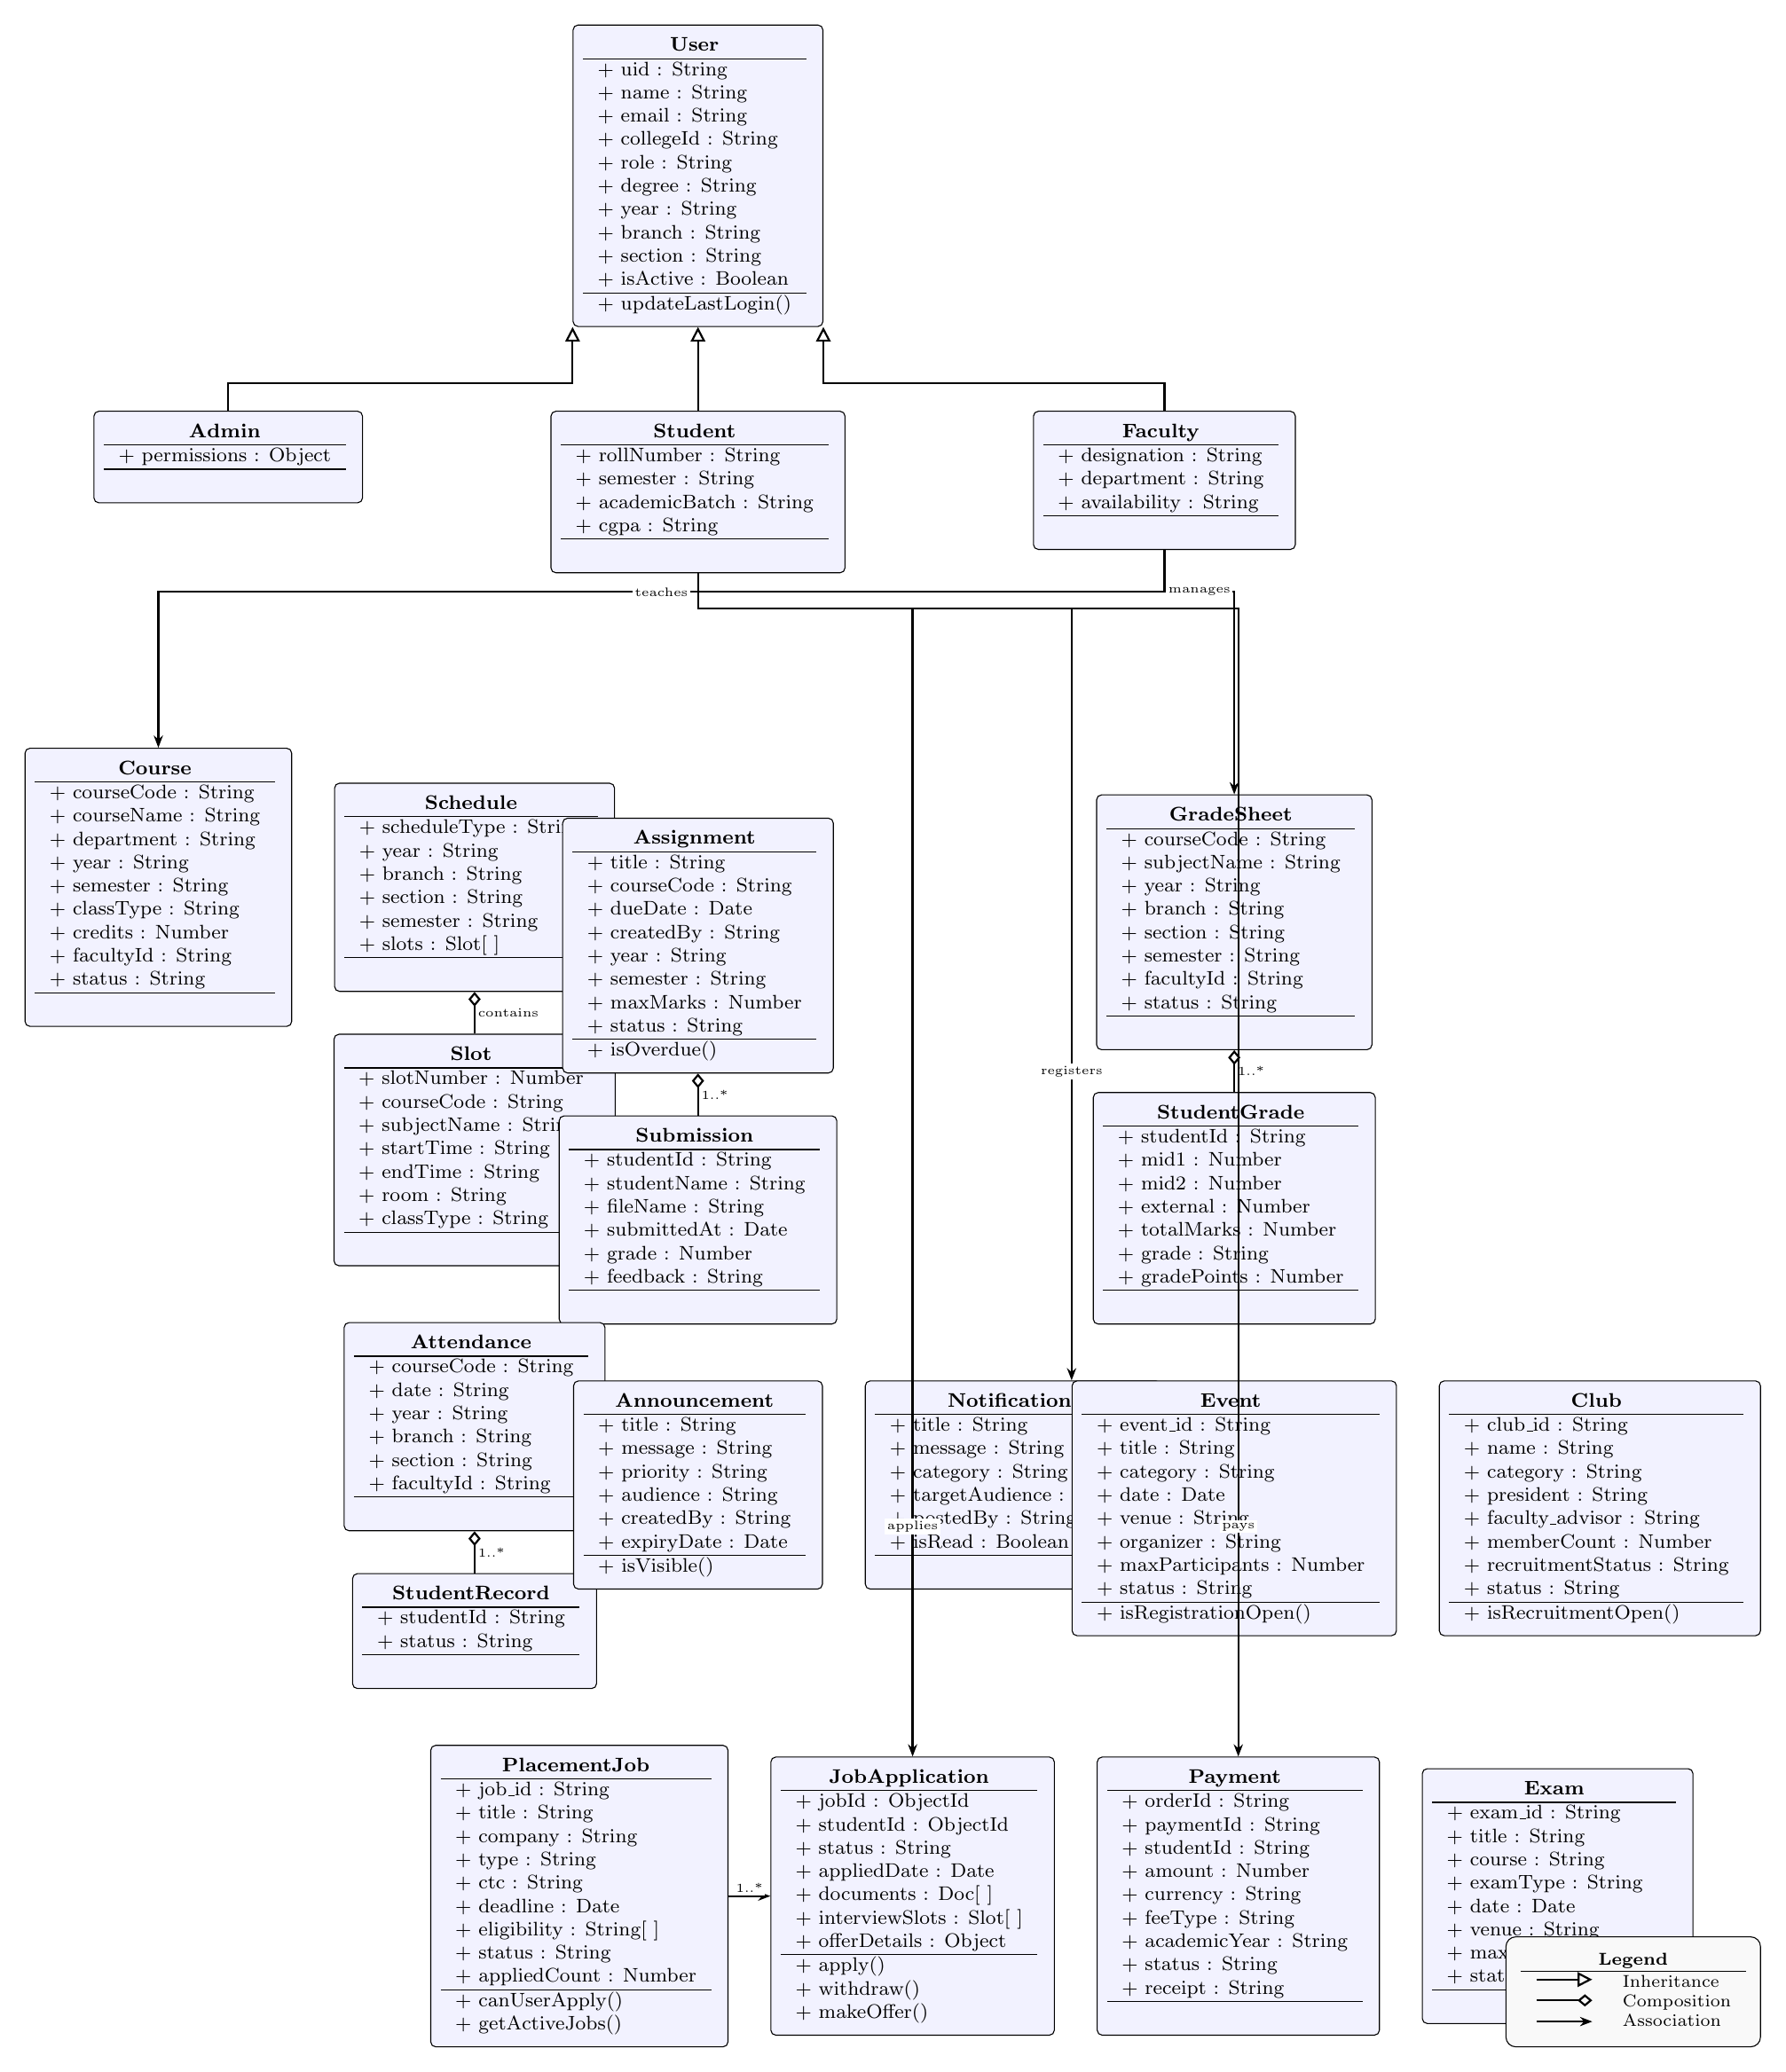
\begin{tikzpicture}[node distance=6mm and 8mm, every node/.style={font=\footnotesize}]

% ══════════════════════════════════════════
%  ROW 1 — USERS (center top)
% ══════════════════════════════════════════
\node[class] (User) {
  \begin{tabular}{l}
    \multicolumn{1}{c}{\textbf{User}} \\ \hline
    + uid : String \\
    + name : String \\
    + email : String \\
    + collegeId : String \\
    + role : String \\
    + degree : String \\
    + year : String \\
    + branch : String \\
    + section : String \\
    + isActive : Boolean \\ \hline
    + updateLastLogin() \\
  \end{tabular}
};

\node[class, below left=12mm and 30mm of User] (Admin) {
  \begin{tabular}{l}
    \multicolumn{1}{c}{\textbf{Admin}} \\ \hline
    + permissions : Object \\ \hline
    \\
  \end{tabular}
};

\node[class, below=12mm of User] (Student) {
  \begin{tabular}{l}
    \multicolumn{1}{c}{\textbf{Student}} \\ \hline
    + rollNumber : String \\
    + semester : String \\
    + academicBatch : String \\
    + cgpa : String \\ \hline
    \\
  \end{tabular}
};

\node[class, below right=12mm and 30mm of User] (Faculty) {
  \begin{tabular}{l}
    \multicolumn{1}{c}{\textbf{Faculty}} \\ \hline
    + designation : String \\
    + department : String \\
    + availability : String \\ \hline
    \\
  \end{tabular}
};

% Inheritance arrows
\draw[inherit] (Admin.north) -- ++(0,0.4) -| (User.south west);
\draw[inherit] (Student.north) -- (User.south);
\draw[inherit] (Faculty.north) -- ++(0,0.4) -| (User.south east);

% ══════════════════════════════════════════
%  ROW 2 — LEFT: Course / Schedule
% ══════════════════════════════════════════
\node[class, below=35mm of Admin, xshift=-10mm] (Course) {
  \begin{tabular}{l}
    \multicolumn{1}{c}{\textbf{Course}} \\ \hline
    + courseCode : String \\
    + courseName : String \\
    + department : String \\
    + year : String \\
    + semester : String \\
    + classType : String \\
    + credits : Number \\
    + facultyId : String \\
    + status : String \\ \hline
    \\
  \end{tabular}
};

\node[class, right=6mm of Course] (Schedule) {
  \begin{tabular}{l}
    \multicolumn{1}{c}{\textbf{Schedule}} \\ \hline
    + scheduleType : String \\
    + year : String \\
    + branch : String \\
    + section : String \\
    + semester : String \\
    + slots : Slot[ ] \\ \hline
    \\
  \end{tabular}
};

\node[class, below=6mm of Schedule] (Slot) {
  \begin{tabular}{l}
    \multicolumn{1}{c}{\textbf{Slot}} \\ \hline
    + slotNumber : Number \\
    + courseCode : String \\
    + subjectName : String \\
    + startTime : String \\
    + endTime : String \\
    + room : String \\
    + classType : String \\ \hline
    \\
  \end{tabular}
};

% Faculty --> Course
\draw[assoc] (Faculty.south) -- ++(0,-0.6) -| node[label style, pos=0.25]{teaches} (Course.north);
% Schedule *-- Slot
\draw[compose] (Slot.north) -- node[label style, right]{contains} (Schedule.south);

% ══════════════════════════════════════════
%  ROW 2 — CENTER: Assignment / GradeSheet
% ══════════════════════════════════════════
\node[class, below=35mm of Student] (Assignment) {
  \begin{tabular}{l}
    \multicolumn{1}{c}{\textbf{Assignment}} \\ \hline
    + title : String \\
    + courseCode : String \\
    + dueDate : Date \\
    + createdBy : String \\
    + year : String \\
    + semester : String \\
    + maxMarks : Number \\
    + status : String \\ \hline
    + isOverdue() \\
  \end{tabular}
};

\node[class, below=6mm of Assignment] (Submission) {
  \begin{tabular}{l}
    \multicolumn{1}{c}{\textbf{Submission}} \\ \hline
    + studentId : String \\
    + studentName : String \\
    + fileName : String \\
    + submittedAt : Date \\
    + grade : Number \\
    + feedback : String \\ \hline
    \\
  \end{tabular}
};

% Assignment *-- Submission
\draw[compose] (Submission.north) -- node[label style, right]{1..*} (Assignment.south);

% ══════════════════════════════════════════
%  ROW 2 — RIGHT: Attendance / GradeSheet
% ══════════════════════════════════════════
\node[class, below=35mm of Faculty, xshift=10mm] (GradeSheet) {
  \begin{tabular}{l}
    \multicolumn{1}{c}{\textbf{GradeSheet}} \\ \hline
    + courseCode : String \\
    + subjectName : String \\
    + year : String \\
    + branch : String \\
    + section : String \\
    + semester : String \\
    + facultyId : String \\
    + status : String \\ \hline
    \\
  \end{tabular}
};

\node[class, below=6mm of GradeSheet] (StudentGrade) {
  \begin{tabular}{l}
    \multicolumn{1}{c}{\textbf{StudentGrade}} \\ \hline
    + studentId : String \\
    + mid1 : Number \\
    + mid2 : Number \\
    + external : Number \\
    + totalMarks : Number \\
    + grade : String \\
    + gradePoints : Number \\ \hline
    \\
  \end{tabular}
};

% GradeSheet *-- StudentGrade
\draw[compose] (StudentGrade.north) -- node[label style, right]{1..*} (GradeSheet.south);
% Faculty --> GradeSheet
\draw[assoc] (Faculty.south) -- ++(0,-0.6) -| node[label style, pos=0.25]{manages} (GradeSheet.north);

% ══════════════════════════════════════════
%  ROW 3 — LEFT: Attendance
% ══════════════════════════════════════════
\node[class, below=8mm of Slot] (Attendance) {
  \begin{tabular}{l}
    \multicolumn{1}{c}{\textbf{Attendance}} \\ \hline
    + courseCode : String \\
    + date : String \\
    + year : String \\
    + branch : String \\
    + section : String \\
    + facultyId : String \\ \hline
    \\
  \end{tabular}
};

\node[class, below=6mm of Attendance] (AttRecord) {
  \begin{tabular}{l}
    \multicolumn{1}{c}{\textbf{StudentRecord}} \\ \hline
    + studentId : String \\
    + status : String \\ \hline
    \\
  \end{tabular}
};

\draw[compose] (AttRecord.north) -- node[label style, right]{1..*} (Attendance.south);

% ══════════════════════════════════════════
%  ROW 3 — CENTER: Announcement / Notification
% ══════════════════════════════════════════
\node[class, below=8mm of Submission] (Announcement) {
  \begin{tabular}{l}
    \multicolumn{1}{c}{\textbf{Announcement}} \\ \hline
    + title : String \\
    + message : String \\
    + priority : String \\
    + audience : String \\
    + createdBy : String \\
    + expiryDate : Date \\ \hline
    + isVisible() \\
  \end{tabular}
};

\node[class, right=6mm of Announcement] (Notification) {
  \begin{tabular}{l}
    \multicolumn{1}{c}{\textbf{Notification}} \\ \hline
    + title : String \\
    + message : String \\
    + category : String \\
    + targetAudience : String \\
    + postedBy : String \\
    + isRead : Boolean \\ \hline
    \\
  \end{tabular}
};

% ══════════════════════════════════════════
%  ROW 3 — RIGHT: Event / Club
% ══════════════════════════════════════════
\node[class, below=8mm of StudentGrade] (Event) {
  \begin{tabular}{l}
    \multicolumn{1}{c}{\textbf{Event}} \\ \hline
    + event\_id : String \\
    + title : String \\
    + category : String \\
    + date : Date \\
    + venue : String \\
    + organizer : String \\
    + maxParticipants : Number \\
    + status : String \\ \hline
    + isRegistrationOpen() \\
  \end{tabular}
};

\node[class, right=6mm of Event] (Club) {
  \begin{tabular}{l}
    \multicolumn{1}{c}{\textbf{Club}} \\ \hline
    + club\_id : String \\
    + name : String \\
    + category : String \\
    + president : String \\
    + faculty\_advisor : String \\
    + memberCount : Number \\
    + recruitmentStatus : String \\
    + status : String \\ \hline
    + isRecruitmentOpen() \\
  \end{tabular}
};

% Student --> Event
\draw[assoc] (Student.south) -- ++(0,-0.5) -| node[label style, pos=0.8]{registers} (Event.north west);

% ══════════════════════════════════════════
%  ROW 4 — Placement & Payment
% ══════════════════════════════════════════
\node[class, below=8mm of AttRecord, xshift=15mm] (PlacementJob) {
  \begin{tabular}{l}
    \multicolumn{1}{c}{\textbf{PlacementJob}} \\ \hline
    + job\_id : String \\
    + title : String \\
    + company : String \\
    + type : String \\
    + ctc : String \\
    + deadline : Date \\
    + eligibility : String[ ] \\
    + status : String \\
    + appliedCount : Number \\ \hline
    + canUserApply() \\
    + getActiveJobs() \\
  \end{tabular}
};

\node[class, right=6mm of PlacementJob] (JobApp) {
  \begin{tabular}{l}
    \multicolumn{1}{c}{\textbf{JobApplication}} \\ \hline
    + jobId : ObjectId \\
    + studentId : ObjectId \\
    + status : String \\
    + appliedDate : Date \\
    + documents : Doc[ ] \\
    + interviewSlots : Slot[ ] \\
    + offerDetails : Object \\ \hline
    + apply() \\
    + withdraw() \\
    + makeOffer() \\
  \end{tabular}
};

\node[class, right=6mm of JobApp] (Payment) {
  \begin{tabular}{l}
    \multicolumn{1}{c}{\textbf{Payment}} \\ \hline
    + orderId : String \\
    + paymentId : String \\
    + studentId : String \\
    + amount : Number \\
    + currency : String \\
    + feeType : String \\
    + academicYear : String \\
    + status : String \\
    + receipt : String \\ \hline
    \\
  \end{tabular}
};

\node[class, right=6mm of Payment] (Exam) {
  \begin{tabular}{l}
    \multicolumn{1}{c}{\textbf{Exam}} \\ \hline
    + exam\_id : String \\
    + title : String \\
    + course : String \\
    + examType : String \\
    + date : Date \\
    + venue : String \\
    + maxMarks : Number \\
    + status : String \\ \hline
    \\
  \end{tabular}
};

% PlacementJob --> JobApplication
\draw[assoc] (PlacementJob.east) -- node[label style, above]{1..*} (JobApp.west);
% Student --> JobApplication
\draw[assoc] (Student.south) -- ++(0,-0.5) -| node[label style, pos=0.9]{applies} (JobApp.north);
% Student --> Payment
\draw[assoc] (Student.south) -- ++(0,-0.5) -| node[label style, pos=0.9]{pays} (Payment.north);

% ══════════════════════════════════════════
%  LEGEND (bottom right)
% ══════════════════════════════════════════
\node[draw, rounded corners, fill=gray!5, inner sep=6pt,
      anchor=south east, font=\scriptsize]
  at (current bounding box.south east) {
  \begin{tabular}{ll}
    \multicolumn{2}{c}{\textbf{Legend}} \\ \hline
    \tikz\draw[inherit] (0,0) -- (0.8,0); & Inheritance \\
    \tikz\draw[compose] (0,0) -- (0.8,0); & Composition \\
    \tikz\draw[assoc]   (0,0) -- (0.8,0); & Association \\
  \end{tabular}
};

\end{tikzpicture}

\end{document}
